\section{Auswertung}

Im Folgenden werden die erhobenen Messdaten ausgewertet um die Polarisation,
die Grundmode, die erste angeregte Mode, die Wellenlänge sowie die Stabilitätsmessung
des $\ce{HeNe}$-Lasers zu erhalten.

\subsection{Polarisationsmessung}
\label{sec:pol}

Die Messdaten sind in Tab. \ref{tab:pol} dargestellt. Die Intensität $I(\varphi)$
ist in Abhängigkeit des Winkels des Polarisationsfilters $\varphi$ gemessen worden.

Die Messdaten sind an eine Funktion der Form:

\begin{equation}
  \label{eqn:Pol}
  I\left(\varphi\right) = I_0\cdot \sin^2\left(\varphi - \varphi_0\right)
\end{equation}

gefittet worden. Die einzelnen Parameter der Ausgleichsrechnung sind in Tab. \ref{tab:aus_pol}
dargestellt.

\begin{table}
\centering
\caption{Parameter der Ausgleichsrechnung zu \eqref{eqn:Pol}}
\label{tab:aus_pol}
\begin{tabular}{S S}
\toprule
{Parameter} & {Wert}  \\
\midrule
$I_\text{0}$  & \text{(}0.29 $\pm$ 0.037\text{)}\text{mA}  \\
$\varphi_\text{0}$ & \text{(}0.75 $\pm$ 0.011\text{)}\text{rad} \\
\bottomrule
\end{tabular}
\end{table}

\begin{figure}[h]
  \centering
  \includegraphics[width = \textwidth]{Pics/Polarisationsmessung.pdf}
  \caption{Polarisationsmessung mit der zugehörigen Ausgleichsfunktion.}
  \label{fig:Pol}
\end{figure}

\FloatBarrier

\subsection{Modenmessung}
\label{sec:tem}

Die Messdaten zu der Grundmode TEM$_{(0,0)}$ und der ersten angeregte Mode
TEM$_{(0,1)}$ sind in Tab. \ref{tab:tem} einzusehen.
Die Daten der Grundmode sind an eine Gaußfunktion der Form:

\begin{equation}
  \label{eqn:gauß}
  I_{(0, 0)}(L) = I_0\exp\left(-2\left(\frac{L - d_0}{\omega}\right)^2\right)
\end{equation}

gefittet worden.
Dabei sind $I_0$, $d_0$ und $\omega$ freie Parameter, die aus dem Fit bestimmt werden.
$I_0$ stellt dabei die Maximalintensität, $d_0$ die Verschiebung in positive Richtung der Abszisse
und $\omega$ den Radius der Fundamentalmode der Gaußverteilung dar. Der Parameter
$L$ ist die Verschiebung der Photodiode senkrecht zur Strahlebene.

\begin{figure}[h]
  \centering
  \includegraphics[width = \textwidth]{Pics/Grundmode.pdf}
  \caption{Grundmode mit der zugehörigen Ausgleichsfunktion.}
  \label{fig:Grundmode}
\end{figure}

Hingegen sind die Daten der TEM$_{(0,1)}$ an eine doppelte asymmetrische Gaußkurve
für veschiedene Peakintensitäten $I\ua{0,i}$ gefittet worden.
Die Ausgleichsfunktion besitzt folgenden Gestalt:

\begin{equation}
  \label{eqn:doppelter_gauß}
  I_{(0, 1)}(L) = I_{0,1}\exp\left(-2\left(\frac{L - d_{0,1}}{\omega_1}\right)^2\right)
  + I_{0,2}\exp\left(-2\left(\frac{L - d_{0,2}}{\omega_2}\right)^2\right).
\end{equation}

Die Parameter $I\ua{0,i}$, $d\ua{0,i}$ und $\omega\ua{i}$ haben dabei dieselbe Bedeutung,
wie bei der Grundmode. Dabei sind alle Parameter mit i $ = 1$ auf das erste und alle
parameter mit i $ = 2$ auf das zweite Maxima bezogen.
Die Parameter der Ausgleichsrechnungen sind in Tab. \ref{tab:moden} aufgeführt.

\begin{table}
\centering
\caption{Parameter der Ausgleichsrechnung zu den Gleichungen \eqref{eqn:gauß} und \eqref{eqn:doppelter_gauß}}
\label{tab:moden}
\begin{tabular}{S S S}
\toprule
{Parameter} & {Wert} & {Fehler} \\
\midrule
$I_\text{0}$  & 6.08\text{ mA} & 0.079\text{ mA} \\
$\text{$d$}_\text{0}$ & 10.77\text{ mm} & 0.063\text{ mm} \\
$\omega$ & 8.396\text{ mm} & 0.13\text{ mm} \\
$I_\text{0,1}$ & 0.65\text{ }$\mu$\text{A} & 0.035\text{ }$\mu$\text{A} \\
$\text{$d$}_\text{0,1}$ & 4.68\text{ mm} & 0.175\text{ mm} \\
$\omega_\text{1}$ & 5.63\text{ mm} & 0.375\text{ mm} \\
$I_\text{0,2}$ & 0.45\text{ }$\mu$\text{A} & 0.011\text{ }$\mu$\text{A} \\
$\text{$d$}_\text{0,2}$ & 18.61\text{ mm} & 0.089\text{ mm} \\
$\omega_\text{2}$ & 6.46\text{ mm} & 0.189\text{ mm} \\
\bottomrule
\end{tabular}
\end{table}

Mit der Funktion \eqref{eqn:doppelter_gauß} und den Parametern aus Tab. \ref{tab:moden}
ergibt sich die Ausgleichskurve zu dem in Abb. \ref{fig:moden} dargestellten Plot.

\begin{figure}[h]
  \centering
  \includegraphics[width = \textwidth]{Pics/erste_angeregte_Mode.pdf}
  \caption{Erste angeregte Mode mit der zugehörigen Ausgleichsfunktion.}
  \label{fig:moden}
\end{figure}

\FloatBarrier

\subsection{Wellenlängenmessung}
\label{sec:wellenlänge}

Die Messdaten zu der Wellenlängenmessung ist in Tab. \ref{tab:wellenlänge}
dargestellt.
Die Wellenlänge wird durch Formel \eqref{eqn:wellenlänge} berechnet.

\begin{equation}
  \label{eqn:wellenlänge}
  \lambda = \frac{a}{n}\cdot\sin\left(\tan^-1\left(\frac{d_n}{L}\right)\right)
\end{equation}

Dabei ist $a$ die Gitterbreite, $d_n$ der Abstand der Hauptmaxima zu dem zentralen
Hauptmaxima, $L$ der Abstand des Schirms von dem Spalt und $n$ die Ordnung der
Hauptmaxima. Die Ordnung des Hauptmaximums wird wie in Abb. \ref{fig:ordnung}
dargestellt bestimmt.

\begin{figure}[h]
  \centering
  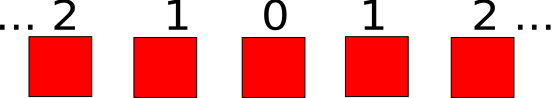
\includegraphics[width = 0.5\textwidth]{Pics/Ordnung.pdf}
  \caption{Schema zum Ablesen der Ordnung der Hauptmaxima.}
  \label{fig:ordnung}
\end{figure}

Dabei hat das zetrale Hauptmaxima die Ordnung 0.
Das verwendete Gitter hat eine Gitterbreite von $a = \frac{1}{100}\si{\milli\meter}$
und der Abstand zum Schirm beträgt $L = \SI{75.7}{\centi\meter}$. Als Ablesefehler
der Abstände der Hauptmaxima wird $\delta L = \SI{0.05}{\centi\meter}$ angenommen.

\begin{table}
\centering
\caption{Messdaten zur Wellenlängenmessung.}
\label{tab:wellenlänge}
\begin{tabular}{S S S @{${}\pm{}$} S}
\toprule
{Parameter} & {Wert in $\si{\centi\meter}$} & \multicolumn
{2}{c}{$\lambda$ in $\si{\nano\meter}$} \\
\midrule
$H_\text{-2}$  & 9.8 & 641.94 & 3.22 \\
$H_\text{-1}$ & 4.9 & 645.94  & 6.56 \\
$H_\text{1}$ & 5.1 & 672.18 & 6.56 \\
$H_\text{2}$ & 9.7 & 635.49 & 3.22 \\
\bottomrule
\end{tabular}
\end{table}

Gemittelt über die Anzahl ergeben die Wellenlängen
aus Tab. \ref{tab:wellenlänge} die beste Schätzung $\lambda\ua{He-Ne} = \SI{648.9(26)}{\nano\meter}$.

\FloatBarrier

\subsection{Stabilitätsmessung}
\label{sec:stabilitätsmessung}

Die Messdaten der Stabilitätsmessung des $\ce{He-Ne}$-Lasers für die verschiedenen
Resononatoren sind in in Tab. \ref{tab:kk} und Tab. \ref{tab:kp} dargestellt.

Die Messdaten des Resonators mit der Spiegelkombination konkav-konkav
sind an eine quadratische Funktion mit den Paramtern $a, b$ und $c$ gefittet (vgl. \eqref{eqn:quad}).

\begin{equation}
  \label{eqn:quad}
  I\ua{quad}\left(L\right) = a\cdot L^2 + b\cdot L + c
\end{equation}

Aus der Ausgleichsrechnung ergeben sich die Parameter zu:

\begin{align}
  \label{eqn:params_kk}
  a =& \SI{-7.68(928)e-6}{\milli\ampere\per\centi\meter^2}\\
  b =& \SI{3.57(175)e-3}{\milli\ampere\per\centi\meter}\\
  c =& \SI{-6.83(807)e-2}{\milli\ampere}.
\end{align}

Hingegen werden die Messdaten des Resonators mit der Spiegelkombination konkav-planar
an eine lineare Funktion mit den Parametern $a$ und $b$ gefittet (vgl. \eqref{eqn:lin}).

\begin{equation}
  \label{eqn:lin}
  I\ua{lin}\left(L\right) = a\cdot L + b
\end{equation}

Die Parameter der Ausgleichsrechnung der Funktion \eqref{eqn:lin} ergeben sich zu:

\begin{align}
  \label{eqn:params_kp}
  a =& \num{-6.71(89)e-2}\frac{\mu\si{\ampere}}{\si{\centi\meter}}\\
  b =& \num{6.52(61)}\mu\si{\ampere}
\end{align}

Die dazugehörigen Diagramme sind in Abb. \ref{fig:stabilität_quad} und Abb. \ref{fig:stabilität_lin}
dargestellt.

\begin{figure}[h]
  \centering
  \includegraphics[width = \textwidth]{Pics/Stabilitaet_kk.pdf}
  \caption{Messdaten und Fit der Stabilitätsmessung des Resonators mit der Spiegelkombination konkav-konkav.}
  \label{fig:stabilität_quad}
\end{figure}

\begin{figure}[h]
  \centering
  \includegraphics[width = \textwidth]{Pics/Stabilitaet_kp.pdf}
  \caption{Messdaten und Fit der Stabilitätsmessung des Resonators mit der Spiegelkombination konkav-planar.}
  \label{fig:stabilität_lin}
\end{figure}

\section{Diskussion}

In diesem Kapitel werden die Messergebnisse diskutiert.
Für die Polarisationsmessung wird ein $\sin^2(\varphi)$-Verlauf erwartet, da
das Licht, welches von dem Laser emitiert wird bereits linearpolarisiert ist.
Linear polarisiertes Licht wird durch eine Sinusfunktion beschrieben. Dieses wird
durch einen linearen Polarisationsfilter gestrahlt, wodurch eine weitere
Sinusfunktion auf das Licht angewendet wird. Die beiden erwähnten Sinusfunktionen
multiplizieren sich auf.
Der Zusammenhang der Polarisationsmessung mit dieser
quadrierten Sinusfunktion ist deutlich erkennbar. Somit konnte die Erwartung durch
die Messung bestätigt werden.
Weiterhin sind die Grundmode und die erste angeregte Mode ausgemessen worden.
Die Grundmode konnte der Erwartung entsprechend durch eine Gaußfunktion präzise beschrieben werden.
Die erste angeregte Mode wird hingegen durch eine asymmetrische doppelte Gaußfunktion
beschrieben. Die Asymmetrie entsteht aufgrund der endlichen Ausdehnung des verwendeten
Golddrahtes. Der Golddraht wirft auf die eine Seite der doppelten Gaußfunktion einen
Schatten, der das Maximum deutlich absenkt.

Die Wellenlängenmessung ergibt $\lambda\ua{He-Ne} = \SI{648.9(26)}{\nano\meter}$.
Dieser Wert liegt im roten Bereich des sichtbaren Lichtes. Der Literaturwert wird
mit $\lambda\ua{lit} = \SI{632,82}{\nano\meter}$ angegeben. Die Diskrepanz der beiden Werte liegt
nicht im Fehlerintervall des experimentell bestimmten Wertes. Dies kann dadurch erklärt
werden, dass zu wenige Messdaten aufgenommen wurden, um einen präzisen Wert zu bestimmen.
Außerdem ist nicht sichergestellt, dass die angegebene Gitterkonstante
$a = \frac{1}{100}\si{\milli\meter}$ bei dem verwendeten Gitter richtig ist.
Daher wird die Diskrepanz auf einen systematischen Fehler und die wenigen Messdaten
zurückgeführt.

Der Vergleich des theoretischen Verlaufes der Stabilitätsmessung und dem gemessenen
Verlauf der konkav-konkav Resonatorspiegelkombination zeigt keine Ähnlichkeit.
Die Intensität des Lasers sollte mit zunehmender Resonantorlänge abnehmen und nicht
wie gemessen zunehmen. Der Verlauf lässt sich nicht durch einen systematischen
Fehler erklären. Die Stabilitätsmessung des konkav-konkaven Spiegelsystems ist
nicht repräsentativ, um die Thoerie zu überprüfen.

Der Verlauf der konkav-planar Resonatorspiegelkombination stimmt hingegen mit der theoretischen
Vorhersage überein.
Das konkav-planar System brachte bei der Vermessung deutliche Probleme mit sich, weil
der $\ce{He-Ne}$-Laser schon bei kleinen Spiegelveränderungen aufgehört hat zu lasern.
Die Messung wurde mehrfach durchgeführt, da teilweise nur 2 Messpunkte aufgenommen
werden konnten, bevor der Laser nicht mehr zum lasern gebracht werden konnte.
Letztendlich sind nur fünf Messpunkte aufgenommen worden, weshalb das
Ergebnis starke statistische Unsicherheiten aufweist. Damit ist die Messung ebenfalls
nicht repräsentativ, um diese mit dem theoretischen Verlauf zu vergleichen.

Die Intensität des Lasers nach der Justage war deutlich
unter $\SI{1}{\milli\ampere}$ und ist bei einigen Messungen auf unter $\SI{1}{\micro\ampere}$
abgefallen. Deshalb wird auf einen systematischen Fehler des Aufbaus geschlossen.
Die niederige Intensität könnte durch die Photodiode hervorgerufen worden sein,
da nicht sichergestellt war, dass der Laserstrahl exakt auf diese eingefallen ist.
Obwohl der Strahlengang mehrfach überprüft wurde, kann es dabei zu dem
systematischen Fehler gekommen sein.

\section{Messdaten}

In diesem Kapitel sind die Messdaten zu den Kapiteln \ref{sec:pol}, \ref{sec:tem}
und \ref{sec:stabilitätsmessung} aufgeführt.


\begin{table}
\centering
\caption{Messdaten der Polarisationsmessung.}
\label{tab:pol}
\begin{tabular}{S S}
\toprule
{$I\ua{Pol}$ in $\si{\milli\ampere}$} & {$\phi$ in  $\si{\degree}$}  \\
\midrule
0.116  & 0\\
0.067  & 10\\
0.034  & 20\\
0.011  & 30\\
0.001  & 40\\
0.004  & 50\\
0.020  & 60\\
0.049  & 70\\
0.086  & 80\\
0.137  & 90\\
0.187  & 100\\
0.238  & 110\\
0.281  & 120\\
0.307  & 130\\
0.308  & 140\\
0.288  & 150\\
0.251  & 160\\
0.198  & 170\\
0.137  & 180\\
0.083  & 190\\
0.040  & 200\\
0.013  & 210\\
0.001  & 220\\
0.005  & 230\\
0.024  & 240\\
0.053  & 250\\
0.094  & 260\\
0.146  & 270\\
0.208  & 280\\
0.264  & 290\\
0.295  & 300\\
0.296  & 310\\
0.279  & 320\\
0.252  & 330\\
0.214  & 340\\
0.167  & 350\\
0.111  & 360\\
\bottomrule
\end{tabular}
\end{table}

\begin{table}
\centering
\caption{Messdaten der Modenmessung.}
\label{tab:tem}
\begin{tabular}{S S S }
\toprule
{$I_{(0, 0)}$ in $\mu\si{\ampere}$} & {$I_{(0, 1)}$ in $\mu\si{\ampere}$} & {$\Delta L$ in $\si{\milli\meter}$}  \\
\midrule
0.12  & 0.23  & 0\\
0.26  & 0.33  & 1\\
0.47  & 0.40  & 2\\
0.90  & 0.49  & 3\\
1.48  & 0.56  & 4\\
2.17  & 0.65  & 5\\
3.28  & 0.66  & 6\\
4.41  & 0.53  & 7\\
4.95  & 0.30  & 8\\
5.79  & 0.15  & 9\\
6.09  & 0.04  & 10\\
5.86  & 0.02  & 11\\
5.48  & 0.03  & 12\\
5.19  & 0.08  & 13\\
4.54  & 0.17  & 14\\
3.76  & 0.26  & 15\\
2.76  & 0.34  & 16\\
2.17  & 0.39  & 17\\
1.55  & 0.43  & 18\\
0.96  & 0.47  & 19\\
0.54  & 0.39  & 20\\
0.32  & 0.32  & 21\\
0.18  & 0.29  & 22\\
\text{\,\,\,\,\,\,\,\,\,\,\,\,\,\,\,\,--}  & 0.19  & 23\\
\text{\,\,\,\,\,\,\,\,\,\,\,\,\,\,\,\,--}  & 0.10  & 24\\
\text{\,\,\,\,\,\,\,\,\,\,\,\,\,\,\,\,--}  & 0.04  & 25\\
\bottomrule
\end{tabular}
\end{table}

\begin{table}
\centering
\caption{Messdaten der Resonatorstabilitätemessung für die Spiegelkombination konkav-konkav.}
\label{tab:kk}
\begin{tabular}{S S}
\toprule
{$\Delta L$ in $\si{\centi\meter}$} & {$I$ in $\si{\milli\ampere}$}  \\
\midrule
67.0  & 0.14\\
72.3  & 0.14\\
77.1  & 0.16\\
82.0  & 0.17\\
87.1  & 0.18\\
91.7  & 0.21\\
97.1  & 0.21\\
102.1  & 0.22\\
107.0  & 0.21\\
112.1  & 0.23\\
122.1  & 0.26\\
\bottomrule
\end{tabular}
\end{table}

\begin{table}
\centering
\caption{Messdaten der Resonatorstabilitätemessung für die Spiegelkombination konkav-planar.}
\label{tab:kp}
\begin{tabular}{S S}
\toprule
{$\Delta L$ in $\si{\centi\meter}$} & {$I$ in $\si{\micro\ampere}$}  \\
\midrule
58.9  & 2.57\\
62.9  & 2.40\\
68.1  & 1.83\\
73.1  & 1.48\\
78.1  & 1.40\\
\bottomrule
\end{tabular}
\end{table}

